\chapter{Theoretical and Technical Background}
\label{ch:background}
In this chapter, we provide a brief introduction to the methods used in this thesis. We keep the discussion as general as possible, as more specific details will be presented in the results section~\ref{sec:results}.
We begin by introducing the forward model in section~\ref{sec:formodel}, which we use to simulate the data. Since the forward model is weakly non-linear, we employ an affine transformation, see section~\ref{sec:affine}, to project the linear model onto the non-linear one, allowing us to treat the problem as a linear inverse problem.
This enables the application of Bayesian inference in section~\ref{sec:bayes}, where we formulate a hierarchical linear-Gaussian model to define and structure the posterior distribution.
For comparison, we briefly present the Tikhonov regularization approach, see section~\ref{sec:regularise}.
In section~\ref{sec:sampling}, we introduce Markov Chain Monte Carlo (MCMC) methods to sample from the posterior distribution.
Finally, in section~\ref{sec:tensortrain}, instead of sampling, we can approximate the posterior distribution using the tensor train format.


\section{Forward Model}
\label{sec:formodel}
The forward model is based on a satellite measuring through the amtosphere, known as limb sounding, as shown in Figure~\ref{fig:FirstLIMB}.
One measurement $y_j$ of a stationary satellite can be describes as the path integral through the atmosphere along the line of sight, for $j=1,2,\ldots,m$.
For each measurement we can define a tangent height $h_{\ell_j}$ as the shortest distance along the line of sight to the earth.

\begin{figure}[ht!]
	\centering
	\scalebox{0.9}{\input{FirstLIMB.pdf_tex}}
	\caption{This figure illustrates a limb sounding measurement setup, specifically how the line of sight of a satellite at altitude $h_{\text{obs}}$ is partitioned according to a discretized atmospheric model. The atmosphere is divided into $n$ layers, allowing the line of sight $\Gamma_j$ to be discretized into segments $\Delta r_i$ for $i = \ell_j, \dots, n$.
	Here, $\ell_j \in \mathbb{N}$ denotes the index corresponding to the tangent height $h_{\ell_j}$ relative to the Earth's radius $R_E$. This setup forms the basis for the numerical solution of the integral in Eq.~\ref{eq:RTE}, known as the radiative transfer equation.}
	\label{fig:FirstLIMB}
\end{figure}

The $j^\text{th}$ measurement, is modelled by the radiative transfer equation (RTE)~\cite{mipas2000handbook}
\begin{align}
	\label{eq:RTE} 
	y_j =   \int_{\Gamma_j}  B(\nu,T) k(\nu, T)   \frac{p(T)}{k_{\text{B}} T(r)}  x(r)  \tau(r) \text{d}r + \eta_j \, \\
	\tau(r) = \exp{ \Bigl\{ - \int^{r}_{r_\text{obs}}  k(\nu, T)   \frac{p(T)}{k_B T(r^{\prime})}  x(r^{\prime}) \text{d}r^{\prime} \Bigr\} }
\end{align}
where the path from the satellite along the line-of-sight of the $j^\text{th}$ pointing direction is $\Gamma_j$ and the ozone concentration at distance $r$ from the radiometer is $x(r)$ plus some noise $\eta_j$.
Within the stratosphere the number density $p(T) / (k_{\text{B}} T(r))$ of molecules is dependent on the pressure $p(T)$, the temperature $T(r)$, and the Boltzmann constant $k_{\text{B}}$.
The factor $\tau(r)\leq 1$ accounts for re-absorption of the radiation along the line-of-sight, which makes the RTE non linear.
The absorption constant $k(\nu, T)$ for a single gas molecule at a specific wavenumber $\nu$ is given by the HITRAN database \cite{gordon2022hitran2020} and acts as a source function when multiplied with the black body radiation $B(\nu,T)$, given by Planck`s law \cite{rybicki2000rte}.
For fundamentals on the Radiative transfer equation we recommend \cite[Chapter 1]{rybicki2000rte}.
 
To enable Matrix-Vector multiplication, we parametrise the ozone profile as a function of height, discretised into the $n$ values for each of $n$ layers of the discretised atmosphere where the $i^\text{th}$ layer is defined by two spheres of radii  $h_{i-1} < h_{i}$, $i = 1, \dots, n$, with $h_0$ and $h_{n} $.
In between the heights $h_{i-1}$ and $h_{i}$, each of the ozone concentration $x_{i}$, the pressure $p_{i}$, the temperature $T_{i}$, and thermal radiation is assumed to be constant.
Above $h_{n}$ and below $h_0$, the ozone concentration is set to zero, so no signal can be obtained.
Then depending on the parameter of interest, which is either the ozone volume mixing ratio $\bm{x} =\{x_1,x_2,\ldots,x_n\} \in \mathbb{R}^{n}$ or the fraction of pressure and temperature $\bm{p/T}= \{p_1/T_1,p_2/T_2,\ldots,p_n/T_n\} \in \mathbb{R}^{n} $, we can rewrite the integral in Eq.~\eqref{eq:RTE} as e.g. as a vector multiplication $\bm{A_{j}}(\bm{x},  \bm{p},\bm{T}) \, \bm{x} $, where the non-linear absorption $\tau(r)$ is included in $\bm{A_{j}}(\bm{x},  \bm{p},\bm{T})$.
Here, the row vector $\bm{A_{j}}(\bm{x},  \bm{p},\bm{T}) \in \mathbb{R}^{n}$  defines a Kernel for each measurement so that the data vector
\begin{align}
	\bm{y} = \bm{A}(\bm{x},  \bm{p},\bm{T}) \, \bm{x} + \bm{\eta}= \bm{A}(\bm{x},  \bm{p},\bm{T}) \,
	\frac{ \bm{p}}{\bm{T}} + \bm{\eta} \, .
\end{align}
can be written as a matrix vector multiplication, where the matrix $\bm{A}(\bm{x},  \bm{p},\bm{T}) \in \mathbb{R}^{m \times n}$ and the noise vector $\bm{\eta} \in \mathbb{R}^{m}$.

Since the measurement process includes absorption $\tau(r)$ reducing measurements slighty and making the inverse problem weakly non-linear. 
Hence, we can approximate the non-linear forward model $\bm{A}(\bm{x},  \bm{p},\bm{T})$ with a map $\bm{M}$ and the linear forward model $\bm{A}_L$, so that $\bm{A}(\bm{x},  \bm{p},\bm{T}) \approx \bm{M} \bm{A}_L $.
Here, $\bm{A}_{L,j} $ of matrix as $\bm{A}_L \in \mathbb{R}^{m \times n}$ is defined by the linear forward model, where absorption is neglected, e.g. $\tau = 1$. 
Then each entry in the row vector $\bm{A}_{L,j} $ is either defined by $ B(\nu,T) S(\nu, T)   \frac{\bm{p}(T)}{k_{\text{B}} \bm{T}(r)}  \text{d}r$ or $B(\nu,T) S(\nu, T)   \frac{\bm{x}}{k_{\text{B}}}  \text{d}r$, as in Eq.~\eqref{eq:RTE}, depending on the parameter of interest.
This poses a linear inverse problem with the forward map defined by the matrix $\bm{A} = \bm{M} \bm{A}_L$, where $\bm{M}$ is, more specifically, an affine map.


\section{Affine Map}
\label{sec:affine}
An affine map is any linear map in between two vector spaces or affine spaces, where an affine space does not need to preserve a zero origin, see Def. 2.3.1. in \cite{berger2009geometry}.
In other words an affine map does not need to map to the origin of the associated vector space, or is a linear map on vector spaces including translation, or in the words of my supervisor, C. F., an affine map is a Taylor series of first order.
For more information on affine spaces and maps we refer to the books \cite{berger2009geometry, katsumi1994affine}
\begin{figure}[ht!]
	\centering
	\begin{tikzpicture}
		\node[rectnode] at (2,-4) (NL)    {$W$};
		\node[rectnode] at (-2,-4) (L)    {$V$};
		\draw[<-, very thick] (NL.west) -- (L.east); 
		\node[align=center] at (-5.5,-4) (f3) {linear forward model};
		\node[align=center] at (5.5,-4) (f4) {non-linear forward model};
		\node[align=center] at (0,-5) (f5) {$\bm{A}(\bm{x},  \bm{p},\bm{T}) \bm{x}  \approx \bm{M A}_L  \bm{x} = \bm{A x} $ };
		\node[align=center] at (0,-4) (f5) {affine Map \\ $\bm{M}$};
	\end{tikzpicture}
	\caption[Schematics of Affine Map]{Schematics of Affine Map, which approximates the linear forward model to the non-linear forward model.}
\end{figure}

Consequently, we introduce an affine map $ \bm{M}:\bm{A}_L \bm{x} \rightarrow \bm{A}(\bm{x},  \bm{p},\bm{T}) \bm{x}$, which maps the linear forward model $\bm{A}_L \bm{x}$ onto the non-linear forward model $\bm{A}(\bm{x},  \bm{p},\bm{T}) \bm{x}$.
Then the non linear forward model $\bm{A}(\bm{x},  \bm{p},\bm{T}) \approx \bm{M} \bm{A}_L$ is approximated by the affine map $\bm{M}$ and the linear forward model $\bm{A}_L$.
In practise we generate two affine subspaces spaces $V = \big\{ \bm{A}(\bm{x}^{(1)}, \bm{p,T}), \dots ,\bm{A}(\bm{x}^{(m)}, \bm{p,T})\big\} $ and $W = \big\{ \bm{A}_L\bm{x}^{(1)}, \dots ,\bm{A}_L\bm{x}^{(m)}\big\}$ over the same field, with fixed $\bm{p,T}$ and find the mapping in between those.
Here, the parameter $\bm{x}$ is distributed as the posterior distribution $\big\{  \bm{x}^{(1)} , \dots, \bm{x}^{(m)} \big\} \sim \pi(\bm{x}|\bm{\theta},\bm{y})$ conditioned on the hyper-parameters $\bm{\theta}$, according to our Bayesian hierarchical model.


\section{Bayesian Inference}
\label{sec:bayes}
In this section, we introduce the basics of Bayesian inference for a general unknown parameter $\bm{x}$ given observed data
\begin{align}
	\bm{y} = \bm{A} \bm{x} + \bm{\eta},
	\label{eq:LinDat}
\end{align}
based on a linear forward model $\bm{A}$ and additive noise $\bm{\eta}$.
A more advanced Bayesian framework, applied/tailored to the previously introduced forward model, will be developed in Section~\ref{}.





We can visualise the correlation structure between parameters as well as how distributions progress in a measurement process, using a hierarchically ordered directed acyclic graph (DAG), see Figure~\ref{fig:FirstDAG}.
Since any observational process naturally involves random noise, we include this in the DAG and classify the noise variance as a hyper-parameter within $\bm{\theta}$ \cite{fox2016fast}.  
Other hyper-parameters, to which we assign a hyper-prior distribution $\pi(\bm{\theta})$, may influence the parameters $\bm{x}$ either statistically (indicated by solid arrows), as in Figure~\ref{fig:FirstDAG}, or deterministically (indicated by dashed arrows).
Here we incorporate prior knowledge of $\bm{\theta}$ and the parameter $\bm{x}$ by defining $\pi(\bm{\theta})$ and the prior distribution $\pi(\bm{x}|\bm{\theta})$ according to their receptive physical properties or functional dependences.
This is one of the great strength of Bayesian modelling compared to e.g. regularisation, see section \ref{sec:regularise}.
Then the parameter $\bm{x}$ is mapped deterministically through the forward model onto the space of all measurable quantities $\bm{u}$. From this space, we statistically observe the actual data $\bm{y}$, which includes random (statistical) noise as mentioned above.
The distribution of the data conditioned on the  hyper-parameters $\bm{\theta}$ and the parameters $\bm{x}$ is called the likelihood function $\pi(\bm{y}|\bm{\theta},\bm{x})$, which includes information about the measurement process through the forward model.
Then given some observed data, we like to characterise the posterior distribution $\pi(\bm{\theta}, \bm{x}|\bm{y})$ of the underlying parameters and hyper-parameters by reversing the arrows in Figure~\ref{fig:FirstDAG}. 
\begin{figure}[ht!]
	\centering
	\begin{tikzpicture}
	\node[roundnode2] at (0,3.5) (th)    {$\bm{\theta}$};
	\node[roundnode2] at (0,1.5) (x)    {$\bm{x}$};
	\node[roundnode2] at (0,-1.5) (u)    {$\bm{u}$};
	\node[rectnode] at (0,-3.5) (y)    {$\bm{y}$};
	
	\draw[->, very thick] (th.south) -- (x.north); 
	\draw[->, very thick, mydotted] (x.south) -- (u.north); 
	\draw[->, very thick] (u.south) -- (y.north); 
	\draw[->, very thick] (th) edge[bend right=60] (y);  
	
	\node[align=center] at (2.8,3.5) (tht) {$\sim \pi_{\bm{\theta}}(\cdot) $ hyper-parameters};
	\node[align=center] at (2.4,1.5) (xt) {$\sim \pi_{\bm{x}}(\cdot|\bm{\theta}) $ parameters};
	\node[align=center] at (2.25,0) (At) {$\bm{u} = \bm{Ax}$ noise free data};
	\node[align=center] at (3,-1.5) (ut) {space of all measurables};
	\node[align=center] at (2,-3.5) (yt) {$\sim \pi_{\bm{y}}(\cdot|\bm{\theta},\bm{x})$ data};
	\node[align=center] at (-3,0) (nt) {noise};
\end{tikzpicture}
	\caption[Bayesian Inference DAG]{The directed acyclic graph (DAG) for a linear inverse problem visualises statistical dependencies as solid line arrows and deterministic dependencies as dotted arrows.
	The parameters $\bm{x}$ have some statistical dependency of those hyper-parameters $\bm{\theta}$, which are distributed as $\pi(\bm{\theta})$. Then a parameter $\bm{x} \sim \pi_{\bm{x}}(\cdot|\bm{\theta})$ is mapped onto the space of all measurables $\bm{u}=\bm{Ax}$ deterministically through the linear forward model $\bm{A}$.
	From the space of all measurables we observe some data $\bm{y} = \bm{Ax} + \bm{\eta}$, statistically,  so that $\bm{y}\sim \pi_{\bm{y}}(\cdot|\bm{\theta},\bm{x})$ , with naturally some random noise $\bm{\eta} \sim \pi_{\bm{\eta}}(\cdot|\bm{\theta})$.}
	\label{fig:FirstDAG}
\end{figure}

The posterior distribution, our the function of interest, is defined by Bayes theorem
\begin{align}
	\pi(\bm{x},\bm{\theta}|\bm{y}) = \frac{ \pi(\bm{y} | \bm{x}, \bm{\theta} ) \pi(\bm{x}, \bm{\theta})}{\pi(\bm{y})} \, ,
\end{align}
with the prior distribution $\pi(\bm{x}, \bm{\theta}) = \pi(\bm{x}| \bm{\theta}) \pi(\bm{\theta}) $ and the normalising constant $\pi(\bm{y})$.
If the normalising constant is finite and non-zero we approximate the posterior distribution
\begin{align}
	\pi(\bm{x},\bm{\theta}|\bm{y}) \propto \pi(\bm{y} | \bm{x}, \bm{\theta} ) \pi(\bm{x}, \bm{\theta}) \, .
\end{align}
and the expectation of any a function $h(\bm{x}_{\bm{\theta}})$, where $\bm{x}$ may depend on $\bm{\theta}$, is described as 
\begin{align}
	\text{E}_{\bm{x},\bm{\theta}|\bm{y}} [h(\bm{x}_{\bm{\theta}})] =  \underbrace{\int \int   h(\bm{x}_{\bm{\theta}}) \,  \pi(\bm{x}, \bm{\theta} | \bm{y} ) \, \text{d} \bm{x}  \, \text{d} \bm{\theta}}_{\bm{\mu}_{\text{int}}}   \label{eq:expPos} \, ,
\end{align}
which is may a high dimensional integral and computationally not feasible to solve.
Then the sample based Monte Carlo estimate
\begin{align}
	\label{eq:sampMean}
	\text{E}_{\bm{x},\bm{\theta}|\bm{y}} [h(\bm{x}_{\bm{\theta}})] \approx \underbrace{ \frac{1}{N} \sum_{k=1}^{N} h(\bm{x}^{(k)}_{\bm{\theta}})  }_{\bm{\mu}_{\text{samp}}} \, ,
\end{align}
for large enough $N$ (law of large numbers \cite[Chapter 17]{tweedie2009measprob}) is unbiased \cite{roberts2004general}, where the samples $\{\bm{x}^{(k)},\bm{\theta}^{(k)} \}\sim \pi_{\bm{x}, \bm{\theta}}(\cdot|\bm{y})$, for $k = 1, \dots, N$, form a sample set $\mathcal{M} =\{ (\bm{x},\bm{\theta})^{(1)}, \dots ,  (\bm{x},\bm{\theta})^{(N)} \}$.
Furthermore the central limit theorem states that the samples means $ \bm{\mu}^{(i)}_{samp} $, of independent samples sets $\mathcal{M}_i$ for $i = 1, \dots, n$ of any distribution, converge in distribution to a normal distribution so that
\begin{align}
	\sqrt{n} (\bm{\mu}^{(i)}_{\text{samp}} -  \bm{\mu}_{\text{int}} ) \overset{\mathcal{D}}{\longrightarrow} \mathcal{N} (0,\sigma^2) \text{\cite{geyer1992practical}},
\end{align}
and if $\sigma^2 < \infty$ the Monte Carlo error $\bm{\mu}^{(i)}_{\text{samp}} -  \bm{\mu}_{\text{int}} $ is bounded.

Generating those sample set from the posterior distribution proves to be the next problem.
Since the hyper-parameters and parameters tend to be highly correlated, see Rue and Held in \cite{rue2005gaussian} and Appendix \ref{ap:Correlatation}.
One way to work around that is to parameterise $\bm{x}$ using hyper-parameters $\bm{\theta}$ so that $\bm{x}(\bm{\theta})$ or to factorise the posterior distribution
\begin{align}
	\pi(\bm{x}, \bm{\theta}|\bm{y}) = \pi(\bm{x}| \bm{\theta}, \bm{y}) \pi(\bm{\theta}|\bm{y})
\end{align}
into the conditional posterior $\pi(\bm{x}|\bm{\theta}, \bm{y})$ over latent field $\bm{x}$ and the marginal posterior $\pi(\bm{\theta}|\bm{y})$ of the hyper-parameters $\bm{\theta}$.
This is particular beneficial, when $\bm{x}$ is high dimensional, e.g. $\bm{x} \in \mathbb{R}^n$ with $n = 45$, and $\bm{\theta}$ is low dimensional, e.g. two dimensional.
Then by the law of total expectation \cite{champ2022generalizedlawtotalcovariance} Eq. \ref{eq:expPos} becomes
\begin{align}
	\text{E}_{\bm{x}|\bm{y}} [h(\bm{x})] = \text{E}_{\bm{\theta}|\bm{y}}   \big[ \text{E}_{\bm{x}|\bm{\theta},\bm{y}} [h(\bm{x}_{\bm{\theta}})] \big]=  \int 	\text{E}_{\bm{x}| \bm{\theta},\bm{y}}  [h(\bm{x}_{\bm{\theta}})] \,  \pi( \bm{\theta} | \bm{y} )  \, \text{d} \bm{\theta}   \label{eq:MargExpPos} \, ,
\end{align}
where in the case of a linear-Gaussian Bayesian hierarchical model $\text{E}_{\bm{x}| \bm{\theta},\bm{y}}  [h(\bm{x}_{\bm{\theta}})]$ is well defined.

Due to some Gaussian noise $\bm{\eta} \sim \mathcal{N}(0, \bm{\Sigma}(\bm{\theta})) $ we can set up a linear-Gaussian Bayesian hierarchical model
\begin{subequations}
	\begin{align}
		\bm{y}|\bm{x}, \bm{\theta}&\sim \mathcal{N}(\bm{A} \bm{x}, \bm{\Sigma}(\bm{\theta})) \label{eq:likelihood}  \\
		\bm{x}| \bm{\theta} & \sim  \mathcal{N}( \bm{\mu}, \bm{Q}^{-1}(\bm{\theta})  ) \label{eq:xPrior} \\
		\bm{\theta} &\sim  \pi(\bm{\theta}) \label{eq:gammaPrior}\, ,
	\end{align}
	\label{eq:BayMode}
\end{subequations}
with normally distributed likelihood function $\pi(\bm{y}|\bm{x}, \bm{\theta})$ and prior distribution $\pi(\bm{x}| \bm{\theta})$, specified by the noise covariance matrix $\bm{\Sigma}(\bm{\theta})$ and prior precision matrix $\bm{Q}(\bm{\theta})$, modelled via the hyper-prior distribution $\pi(\bm{\theta})$ \cite{fox2016fast}.
The prior mean is $\bm{\mu}$.
This setup allows us to factorise the posterior distribution efficiently and we call this the marginal and then conditional method.

\subsection{Marginal and then Conditional}
\label{subsec:MTC}
For the in Eq. \ref{eq:BayMode} specified linear-Gaussian Bayesian hierarchical model the marginal posterior distribution is given as
\begin{align}
	\pi(\bm{\theta} | \bm{y}) &= \int \pi(\bm{x}, \bm{\theta} | \bm{y}) \diff \bm{x} \\ 
	\label{eq:condHyper}
	&\propto \sqrt{ \frac{ \det( \bm{\Sigma}^{-1} ) \,  \det( \bm{Q}) }{\det( \bm{Q} + \bm{A}^T \bm{\Sigma}^{-1} \bm{A} ) } } \times \exp \Big[ - \frac{1}{2}(\bm{y} -\bm{A \mu})^T \bm{Q}_{\bm{\theta|y}} (\bm{y} -\bm{A \mu}) \Big] \pi(\bm{\theta}) \, ,
\end{align}
with
\begin{align}
	\bm{Q}_{\bm{\theta|y}} = \bm{\Sigma}^{-1} - \bm{\Sigma}^{-1} \bm{A} (\bm{A}^T \bm{\Sigma}^{-1} \bm{A} + \bm{Q} )^{-1} \bm{A}^T \bm{\Sigma}^{-1} \,  ,
\end{align}
see Lemma 2 in \cite{fox2016fast}.
Conditioned on the hyper-parameters $\bm{\theta}$ we can draw samples from the conditional posterior distribution
\begin{align}
	\bm{x}| \bm{\theta}, \bm{y}  \sim \mathcal{N}\big( \underbrace{\bm{\mu} + (\bm{A}^T \bm{\Sigma}^{-1} \bm{A} + \bm{Q} )^{-1} \bm{A}^T \bm{\Sigma}^{-1} (\bm{y} - \bm{A} \bm{\mu})}_{\bm{\mu}_{\bm{x}|  \bm{\theta}, \bm{y}}} , \underbrace{ (\bm{A}^T \bm{\Sigma}^{-1} \bm{A} + \bm{Q} )^{-1}}_{\bm{\Sigma}_{\bm{x}| \bm{y} , \bm{\theta}}} \big) \, 
\end{align}
using the Randomis then optimize (RTO) method, see section \ref{subsec:RTO},
or calculate weighted expectations e.g. $ \text{E}_{\bm{x}|\bm{\theta},\bm{y}} [\bm{x}| \bm{\theta}, \bm{y}] = \bm{\mu}_{\bm{x}| \bm{\theta}, \bm{y} }$ or use Eq. \ref{eq:MargExpPos} to calculate weighted expectations of $\text{E}_{\bm{x}|\bm{\theta},\bm{y}} [\text{Var}(\bm{x}| \bm{\theta}, \bm{y})]  = \bm{\Sigma}_{\bm{x}| \bm{y} , \bm{\theta}}$ with weights given by $\pi(\bm{\theta} | \bm{y} )$.
Note that the noise covariance $\bm{\Sigma}= \bm{\Sigma}( \bm{\theta}) $ and the prior precision $\bm{Q} = \bm{Q}( \bm{\theta})$ are depending on hyper-parameters $\bm{\theta}$.

\section{Regularisation}
\label{sec:regularise}
Another method to find a solution to a linear inverse problem as in Eq. \ref{eq:LinDat} is to find a solution $\bm{x}_{\lambda}$ according to a data misfit norm and a regularisation semi-norm as in \cite{fox2016fast}.
We will discuss the case of Tikhonov regularisation \cite{kaipio2005statinv,tan2016LecNot} as this is the most similar to a linear-Gaussian hierarchial Bayesian model.

For a parameter $\bm{x}$ a linear forward model matrix $\bm{A}$ and some data $\bm{y}$ the data misfit norm
\begin{align}
	\left\lVert \bm{y} - \bm{A}\bm{x} \right\rVert \, 
\end{align}
gives a measure of how good data fits to a mapped parameter $\bm{Ax}$ and the regularisation semi norm 
\begin{align}
	\lambda \left\lVert \bm{T}\bm{x}  \right\rVert
\end{align}
penalises $\bm{x}$ according to $\bm{T}$ and the regularisation parameter $\lambda > 0$.
Given $\lambda$ a regularised solution
\begin{align}
	\bm{x}_{\lambda} = \underset{\bm{x}}{\text{arg min}} \left\lVert \bm{y} - \bm{A}\bm{x}  \right\rVert^2 + \lambda \left\lVert \bm{T}\bm{x} \right\rVert^2
\end{align}
can be found by the derivativ
\begin{align}
&  &\nabla_{\bm{x}} \big\{  (\bm{y} - \bm{A}\bm{x}_{\lambda} )^T  (\bm{y} - \bm{A}\bm{x}_{\lambda})  + \lambda \bm{x}_{\lambda}^T  \bm{T}^T \bm{T} \bm{x}_{\lambda} \big\} &= 0 \\
&\iff &\nabla_{\bm{x}} \big\{ \bm{y}^T \bm{y} + \bm{x}_{\lambda}^T \bm{A}^T  \bm{A}\bm{x}_{\lambda} - \bm{y}^T \bm{A}\bm{x}_{\lambda} - \bm{x}_{\lambda}^T \bm{A}^T   \bm{y}   + \lambda \bm{x}_{\lambda}^T  \bm{T}^T \bm{T} \bm{x}_{\lambda} \big\} & = 0  \\
& \iff& 2\bm{A}^T  \bm{A}\bm{x}_{\lambda} -2 \bm{A}^T   \bm{y}  + 2 \lambda   \bm{T}^T \bm{T} \bm{x}_{\lambda}  & = 0.
\end{align}
Then a regularised solution is given as:
\begin{align}
	(\bm{A}^T  \bm{A} + \lambda   \bm{L} )^{-1} \bm{A}^T   \bm{y}   = \bm{x}_{\lambda}, 
\end{align}
where we can set $\bm{T}^T \bm{T} = \bm{L}$, which is typically matrix approximation of the nth derivative \cite{tan2016LecNot}.
In practise $\bm{x}_{\lambda}$ is calculated for a range of $\lambda$, and is evaluated by the data-misfit norm with respect to the regularised semi-norm so that the best $\bm{x}_{\lambda}$ lays on the point of maximum curvature of a so-called L-Curve \cite{hansen1993use}, which we will show in section \ref{}.


\section{Sampling Methods}
\label{sec:sampling}
In this section we present the sampling methods used in this thesis and show that the methods we use actually draw samples $ \mathcal{M} = \{ (\bm{x}, \bm{\theta} )^{(1)}, \dots, (\bm{x}, \bm{\theta} )^{(k)} , \dots,  (\bm{x}, \bm{\theta})^{(N)} \} \sim \pi(\bm{x},\bm{\theta}| \bm{y}) $ from the desired target distribution so that we can use sample based estimates as in Eq. \ref{eq:sampMean}.
Here $ \mathcal{M}$ is a Markov-Chain, where each sample $ (\bm{x}, \bm{\theta})^{(k)}$ is only depending on the previous sample  $ (\bm{x}, \bm{\theta})^{(k-1)}$ \cite{}.
Markov-chain Monte Carlo methods generates such a chain $\mathcal{M}$ with random (Monte Carlo) proposals $(\bm{x}, \bm{\theta})^{(k)} \sim q( \cdot |(\bm{x}, \bm{\theta})^{(k-1)})$ according to a proposal distribution, where ergodicity of $\mathcal{M}$ is a sufficient criterium to use samples based estimates \cite{tan2016LecNot, roberts2004general}.
The ergodicy theorem in \cite{tan2016LecNot} states that, if an aperiodic and irreducible Markov chain $\mathcal{M}$ is reversible then it converges towards a stationary unique equilibirum distribution $\pi(\bm{x},\bm{\theta}| \bm{y}) $.
In other words if from any state in the chain we can reach any other state in the sampling space and the previous state, and we do not get stuck in periodic loop, then the chain converges towards a stationary distribution.
In practise one can look at the trace $\pi(\bm{x}^{(k)},\bm{\theta}^{(k)}| \bm{y}) $ for $k = 1, \dots, N$ of the samples and eyeball ergodicity.

The sampling methods used in this thesis have proven ergodic properties, so we will cite and refer the reader to the respective documents.

\subsection{Metropolis- within Gibbs sampling}

As introduced in section \ref{subsec:MTC} when using the MTC method will sample seperatly from $\pi(\bm{\theta}| \bm{y})$ and $\pi(\bm{x}|\bm{\theta}, \bm{y}) $.
To sample from $\pi(\bm{\theta}| \bm{y})$ we use a Metropolis-within-Gibbs sampler as in \cite{fox2016fast} and discuss the 2 dimesnional case, as used in this thesis, with $\bm{\theta}  =( \theta_1 , \theta_2) $, where we do a metroplis step in $\theta_1$ deirection and a gibbs stepp in $\theta_2$ direction.
Ergodicity is proven here \cite{roberts2006harris}.

The Metropolis-within-Gibbs algorithm starts with a initial guess $\bm{\theta}^{(t)}$ at $t=0$.
Then, we propose a new sample $\theta_1 \sim q( \theta_1 | \theta^{(t-1)}_1 )$ conditioned on the previous state according to a symmetric proposal distribution $q(\theta_1 | \theta^{(t-1)}_1 ) = q( \theta^{(t-1)}_1|\theta_1 ) $ , which is a special case of the Metropolis-Hastings algorithm \cite{roberts2006harris} and cancels when computing the acceptance probability $\alpha$. We accept and set $ \theta^{(t)}_1 = \theta_1$ with
\begin{align}
\alpha( \theta_1  | \theta_1^{(t-1)}) = \min \left\{ 1, \frac{\pi(\theta_1  | \theta^{(t-1)}_2, \bm{y}) q(\theta_1^{(t-1)} | \theta_1 )  }{\pi(\theta_1^{(t-1)}| \theta_2^{(t-1)}, \bm{y}) q(\theta_1 | \theta_1^{(t-1)})}  \right\}
\end{align}
or reject and keep $\theta^{(t)}_1 = \theta^{(t-1)}_1$, which we do by comparing $\alpha$ to a uniform random number $u \sim \mathcal{U}(0,1)$.
Next, we do a Gibbs step in $\theta_2$ direction, where Gibbs sampling is a special case of the Metropolis-Hastings algorithm with acceptance probaility of 1, and draw the next sample $\theta_2^{(t)} \sim  \pi( \cdot | \theta_1^{(t)} , \bm{y} ) $ conditioned on $\theta_1^{(t)}$ at step $t$.
We reapet this $N$ times and assure convergence independent of the intial sample (irreducibility) as we discard samples after the so-called burn-in period so that we produce a Markov-Chain of length $N - N_{\text{burn-in}}$.


\begin{algorithm}[!ht]
	\caption{Metropolis within Gibbs}
	\begin{algorithmic}[1]
		\STATE Initialize and suppose two dimensional vector \( \bm{\theta}^{(0)}  =( \theta_1^{(0)} , \theta_2^{(0)}  ) \)
		\FOR{ \( k = 1, \dots, N \)}
		\STATE Propose \( \theta_1 \sim q(\cdot   | \theta_1 ^{(t-1)}) = q(\theta_1 ^{(t-1)} |\cdot  ) \)
		\STATE Compute
		\[ \alpha( \theta_1  | \theta_1^{(t-1)}) = \min \left\{ 1, \frac{\pi(\theta_1  | \theta^{(t-1)}_2, \bm{y}) \cancel{q(\theta_1^{(t-1)} | \theta_1 ) } }{\pi(\theta_1^{(t-1)}| \theta_2^{(t-1)}, \bm{y}) \cancel{q(\theta_1 | \theta_1^{(t-1)})} } \right\} \]
		\STATE Draw $u \sim \mathcal{U}(0,1)$
		\IF{$\alpha \geq u$ }
		\STATE Accept and set \( \theta_1^{(t)} = \theta_1 \)
		\ELSE  
		\STATE Reject and keep \(\theta_1^{(t)} = \theta_1^{(t-1)} \)
		\ENDIF
		\STATE Draw \(\theta_2^{(t)} \sim  \pi( \cdot | \theta_1^{(t)} , \bm{y} )\) 
		\ENDFOR
		\STATE Output: $ \bm{\theta}^{(0)}, \dots,  \bm{\theta}^{(k)} , \dots,   \bm{\theta}^{(N)} \sim \pi(\bm{\theta}| \bm{y}) $
	\end{algorithmic}
\end{algorithm}




\subsection{Draw a sample from a multivariate normal distribution \label{subsec:RTO}}

after sampling from $\pi(\bm{\theta}| \bm{y})$ we draw samples from $\pi(\bm{x}|\bm{\theta}, \bm{y}) $ within the MTC scheme.
For Linear Gaussian Bayesian hierarchical model we can draw a sample $\bm{x}$ from the multivariate normal distribution$\pi(\bm{x}|\bm{\theta}, \bm{y})$  using the radomize then optimise (RTO) method \cite{bardsley2012mcmc}.

In doing so we can rewrite the full conditional normal distribution $\pi( \bm{x}| \bm{y} , \bm{\theta} )$ to:
\begin{align}
	\pi(\bm{x}|\bm{y}, \bm{\theta} ) &\propto \pi(\bm{y} | \bm{x} , \bm{\theta} ) \pi(\bm{x}| \bm{\theta}) \\
	&= \exp  \lVert \hat{\bm{A}} \bm{x} - \hat{\bm{y}} \rVert^2 \, ,
\end{align}
where 
\begin{align}
	\label{eq:minimizer}
	\hat{\bm{A}} = 
	\begin{bmatrix}
		\bm{\Sigma}^{-1/2}(\bm{\theta})  \bm{A}\\
		\bm{Q}^{1/2}(\bm{\theta}) 
	\end{bmatrix} \, , \quad \hat{\bm{y}} = 
	\begin{bmatrix}
		\bm{\Sigma}^{-1/2}(\bm{\theta})  \bm{y} \\
		\bm{Q}^{1/2}(\bm{\theta}) \bm{\mu}
	\end{bmatrix} \, \text{\cite{bardsley2014randomize}}.
\end{align}

Then one sample can be computed by minimising the following equation with respect to $\hat{\bm{x}}$ :
\begin{align}
	\bm{x}_i = \arg \min_{\hat{\bm{x}}} \lVert \hat{\bm{A}} \hat{\bm{x}} - ( \hat{\bm{y}} + \bm{b} ) \rVert^2 , \quad \bm{b} \sim \mathcal{N}(\bm{0}, \mathbf{I}) \, ,
\end{align}
where we add a randomised perturbation $\bm{b}$.
Similarly as in section \ref{sec:reg} we can rewrite the argument of Eq. \ref{eq:minimizer} to 
\begin{align}
	\label{eq:RTO}
	(\bm{A}^T \bm{\Sigma}^{-1}(\bm{\theta}) \bm{A}+
	\bm{Q}(\bm{\theta}) ) \bm{x}_i &= \bm{A}^T \bm{\Sigma}^{-1}(\bm{\theta}) \bm{y} +  \bm{Q}(\bm{\theta}) \bm{\mu} + \bm{v}_1 + \bm{v}_2 \,  ,
\end{align}
where we substitute $ - \hat{\bm{A}}^T  \bm{b}  = \bm{v}_1 + \bm{v}_2$ so that $\bm{v}_1 \sim \mathcal{N}(\bm{0}, \bm{A}^T \bm{\Sigma}^{-1}(\bm{\theta}) \bm{A}) $ and $\bm{v}_2 \sim \mathcal{N}(\bm{0}, \bm{Q}(\bm{\theta}) )$ are independent random variables \cite{bardsley2012mcmc, fox2016fast}.


If within the MTC scheme the Markov chain from the marginal posterior is ergodic then with independent samples $\bm{x}^{(k)}$ from the full conditional $\pi(\bm{x}|\bm{\theta}, \bm{y})$ the combined chain $\{  (\bm{x}, \bm{\theta} )^{(1)}, \dots, (\bm{x}, \bm{\theta} )^{(k)} , \dots,  (\bm{x}, \bm{\theta})^{(N)}  \} \sim \pi(\bm{x},\bm{\theta}| \bm{y})$ is ergodic as well \cite{acosta2014markov}.

\subsection{t-walk}
If there is a functional dependency of the parameters $\bm{x}$ and the hyper-parameters $\bm{\theta}$ so that $\bm{x}(\bm{\theta})$ we can use the t-walk algorithm by Christens and Fox on $\pi(\bm{\theta}|\bm{y} )$.
We use the t-walk as a black box sampler, where convergence is guaranteed by construction \cite{christen2010general}.



\section{Numerical Approxiamtion Methods - Tensor Train}
\label{sec:tensortrain}
First we will derive how we find marginal probality distribution funcitons and then give a brief introduction into tensor train format.
Asumme that the triple $(\Omega, \mathcal{F} , \mathbb{P})$ is called a probability space over the whole sample (or parameter) space $\Omega$ with the collection $\mathcal{F}$ of very countable subset $\{ A _n \}_{n\in \mathbb{N}}$ in $\Omega$, so that $A_n \subseteq  \Omega$, and $\mathbb{P}$ is a measure on $\mathcal{F}$. 
We assume $\mathbb{P}$ fullfils the requirements of a probality measure and $\mathcal{F}$ is a $\sigma $-algebra see Appendix \ref{ch:Mesure}.
We call $\mathbb{P}(A)$ the probaility of an event $A \subseteq \mathcal{F}$ 
\begin{align}
	\mathbb{P}(A) = \int_A \diff \mathbb{P} \text{\cite{}}.
\end{align}
We change variables using the Radon-Nikodym theroem \cite{kopp2004measintprob}
\begin{align}
	\mathbb{P}(A) = \int_{A}  \frac{\diff \mathbb{P}}{\diff x} \diff x = \int_{A}  \pi(x) \diff x
\end{align}
where $\diff x$ is a measure on the same probality space, also known as the lebesgue measure and $\frac{\diff \mathbb{P}}{\diff x}$ is often called Radon-Nikodym derivativ of $\mathbb{P}$ with repect to $x$.
We can say that $\mathbb{P}$ has a density $ \pi(x)$, with repect to $x$ \cite[Chapter 10]{simonnet1996measprob}.
Next, we can define $x: \Omega \longrightarrow X$ as a random variable connecting to the measurable space $(X,\mathcal{X})$ through the probability density function $ \pi(x)$ \cite{kopp2004measintprob}.
For a $d$-dimensional $x$ we call the cartesioan product $\mathcal{X} = \mathcal{X}_1 \times \mathcal{X}_2 \times \dots \times \mathcal{X}_d$ the parameter space in $X$.
If $X = \mathbb{R}^d$ every subset $\mathcal{X}_k \subseteq \mathbb{R}$, for $k = 1, \dots , d$, and $x = (x_1 , \dots ,x_d)$, with $x_k \in \mathcal{X}_k$, $\pi(x)$ is the joint probaility density.
The marginal function
\begin{align}
	f_{X_k}(x_k) = \int_{\mathcal{X}_1} \cdots \int_{\mathcal{X}_d} \uplambda(x) \pi(x) \diff x_1 \cdots \diff x_{k-1} \diff x_{k+1} \cdots \diff x_d \, ,
\end{align}
of an event $x_k$ in $X_k \subseteq X$ is calculated by integrating the probility desnity funciton $\pi(x)$ over the parameter space in all other dimensions.
Here we intrdouce a weight function $\uplambda(x) $ \cite{davis2007methods}, which can be helpful for qraudrature rules.
Cui et al. \cite{cui2022deep} call $\uplambda(x)$ the ' product-from Lebsegue measurable weighting functions" and define it as $\uplambda( \mathcal{X}) = \prod_{i = 1}^{d}  \uplambda_i( \mathcal{X}_i) $ and  $\uplambda_i( \mathcal{X}_i) = \int_{ \mathcal{X}_i} \uplambda_i (x_i) \text{d}x_i$.

Using the tensor train (TT) format we can approximate $d$-dimensional function $\pi(x)$ and compute marginal probailty functions distributions cheaply.
In doing so we have to define a d-dimesnional discrete univariate grid in the parameter space $\mathcal{X}$ with $n$ grid points in each direction.
Then, as the name suggest the tensor train format is a train of tensors which represent this d-dimesnional grid.
More specifically each tensor is a two and three dimensional matrix, which we call core, $\pi_{k} \in \mathbb{R}^{r_{k-1} \times n \times r_{k}}$ and connected with the neighbouring tensor through ranks $r_{k}$ and $r_{k-1}$ for each $k = 1, \dots , d$, as in Figure \ref{fig:TTfig} displayed.
For the first and last dimensional the core outer ranks are $r_0  = r_d = 1$, so that for $x = {x_1, \dots, x_d}$ the function value $\pi(x) = \big( \pi_1(x_1) \dots \pi_d(x_d) \big)\in \mathbb{R}$ is a vector-matrix-vector multiplication and each core $\pi_k(x_k)$ at a fixed $x_k$ on the approximated grid has dimensions $r_{k-1} \times 1 \times r_{k} =r_{k-1} \times r_{k}$.


\begin{figure}[ht!]
	\centering
\begin{subfigure}{\textwidth}
	\input{TTSchem.pdf_tex}
	%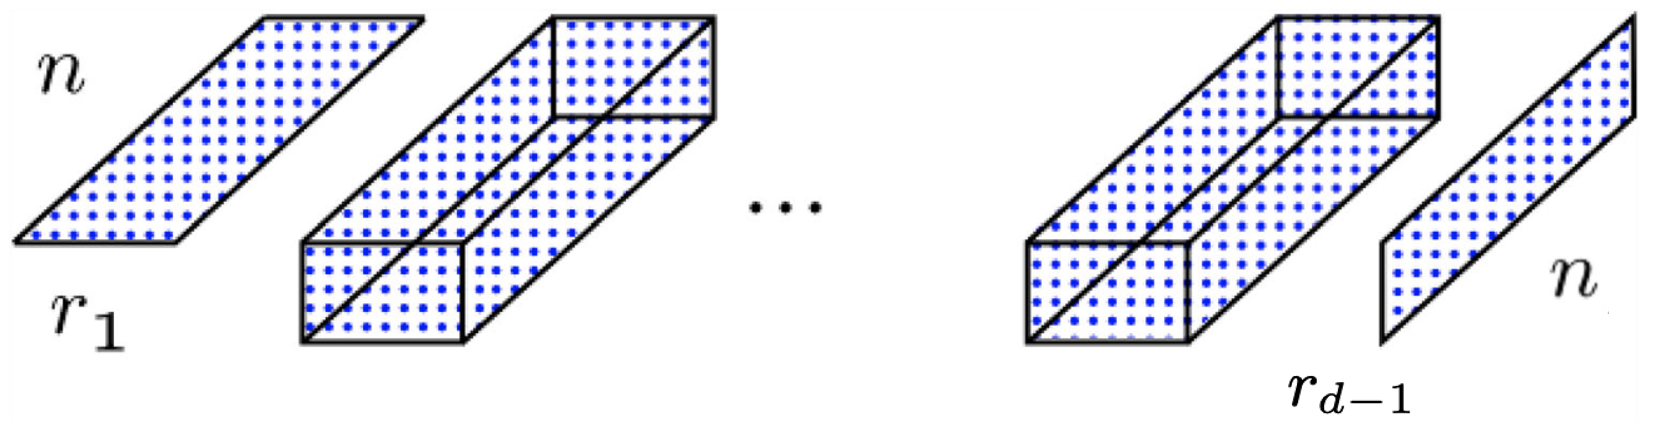
\includegraphics[width = \textwidth]{Figures/TTSchem.png}
	\caption{}
\end{subfigure}
	\centering
\begin{subfigure}{\textwidth}
\begin{tikzpicture} 
	\node[rectnode] at (-5,0) (T1)    {$1 \times n \times r_1$};
	\node[rectnode] at (-2,0) (T2)    {$r_1 \times n \times r_{2}$};
	
	\node[rectnode] at (3,0) (Tn1)    {$r_{d-2} \times n \times r_{d-1} $};
	\node[rectnode] at (6.75,0) (Tn)    {$r_{d-1} \times n \times 1$};
	\draw[-, very thick] (T1.east) -- (T2.west); 
	\draw[-, very thick] (Tn.west) -- (Tn1.east); 
	\draw[-, mydotted, very thick] (T2.east) -- (Tn1.west);
	
	\node[align=center] at (-3.5,0.25) (R) {$r_1$};
	\node[align=center] at (5,0.25) (R) {$r_{d-1}$};	
\end{tikzpicture} 
	\caption{}
\end{subfigure}
\caption[Visualization of Tensor Train cores]{Here we visualize the tensor train cores as two and three dimesnional matrices. Each matrix has a length $n$ according to the gridsize and ther cores are connected through ranks $r$. More specifiaclly a core $\pi_k$ has dimesnions $r_{k-1} \times  n \times r_k$, where $r_0 = r_d = 1$. Figure (a) is taken from \cite{fox2021grid}.}
\label{fig:TTfig}
\end{figure}


Consequently, using a tensor train approxiamtion, the marginal target function
\begin{align}
	\begin{split}
	f_{X_k}(x_k) = \frac{1}{z}
	\Big|  &\left( \int_{\mathbb{R}} \uplambda_1(x_1) \pi_{1}(x_1)\text{d}x_{1} \right) \cdots \left( \int_{\mathbb{R}} \uplambda_{k-1}(x_{k-1}) \pi_{k-1}(x_{k-1}) \text{d}x_{k-1} \right) \\ & \qquad \uplambda_k(x_{k}) \pi_{k}(x_k) \\ &\quad \left( \int_{\mathbb{R}} \uplambda_{k+1}(x_{k+1}) \pi_{k+1}(x_{k+1})\text{d}x_{k+1} \right) \cdots  \left( \int_{\mathbb{R}} \uplambda_d(x_{d}) \pi_{d}(x_d)\text{d}x_d \right) \Big| \, 
	\end{split} 
\end{align}  
is given by integration over each core \cite{dolgov2020approximation} including some normalising constant $z$ \cite{cui2022deep}.
\\


%%%%%% Squared and Basis Function %%%%%
From here we follow the notation and procedure mostly from Cui et al. \cite{cui2022deep} and approximate the square root
\begin{align}
	\sqrt{\pi(x)} \approx g(x) = \bm{G}_1(x_1), \dots ,  \bm{G}_k(x_k), \dots ,  \bm{G}_d(x_d)
\end{align}
for numerical stability, where each TT-core
\begin{equation}
	G^{(\alpha_{k-1},\alpha_k)}_k(x_k) = \sum_{i=1}^{n_k} \phi^{(i)}_k(x_k) \bm{A}_k[\alpha_{k-1}, i, \alpha_k], \quad k = 1, ..., d,
\end{equation}
is associated $k$th coefficient tensor $\bm{A}_k \in \mathbb{R}^{r_{k-1} \times n_k \times r_k}$ and the $k$-th  basis functions $\phi^{(i)}_k(x_k)$.
We assume the function
\begin{align}
	\pi(x) \approx \gamma^{\prime} + g^2(x) \, ,
\end{align} 
is approximated through the TT decomposition $g(x)$, where the error $\gamma^{\prime}$ assures positivity and is chosen according to the $L_2$ norm 
\begin{align}
	\gamma^{\prime} \leq \frac{1}{\uplambda( \mathcal{X})} \lVert g - \sqrt{\pi}\rVert^2_2 \, .
\end{align}
Then the normalised target function is
\begin{align}
	f_X(x) = \frac{1}{z} \pi(x) \uplambda(x) = \frac{1}{z} ( \gamma^{\prime} \uplambda(x) + g^2(x) \uplambda(x)) \, .
\end{align} 
Given the tensor train approximation of the sqared rooted function $\sqrt{\pi}$ can be expressed as
\begin{align}
	\begin{split}
		f_{X_k}(x_k) = \frac{1}{z}  \Bigg( \gamma^{\prime}& \prod_{i=1}^{k-1} \uplambda_i(\mathcal{X}_i) \prod_{i=k+1}^{d} \uplambda_i(\mathcal{X}_i) \\&+  \left( \int_{\mathbb{R}} \bm{G}^2_{1}(x_1) \uplambda_1(x_1)\text{d}x_{1} \right) \cdots \left( \int_{\mathbb{R}} \bm{G}^2_{k-1}(x_{k-1}) \uplambda_{k-1}(x_{k-1}) \text{d}x_{k-1} \right) \\ & \bm{G}^2_{k}(x_k)\uplambda_k(x_{k})\\ & \left( \int_{\mathbb{R}}  \bm{G}^2_{k+1}(x_{k+1})\uplambda_{k+1}(x_{k+1})\text{d}x_{k+1} \right) \cdots  \left( \int_{\mathbb{R}} \bm{G}^2_{d}(x_d)\uplambda_d(x_{d})\text{d}x_d \right) \Bigg) \, .
	\end{split} 
\end{align}

To efficiently calculate these marginals on can use a procedure similar to something that is called left and right orthogonalisation of cores \cite{oseledets2011tensor}.
To do so we define the mass matrix $\bm{M}_k \in \mathbb{R}^{n_k \times n_k}$ by
\begin{equation}
	\bm{M}_k[i, j] = \int_{X_k} \phi^{(i)}_k(x_k) \phi^{(j)}_k(x_k)  \uplambda(x_k) \,dx_k, \quad i = 1, ..., n_k, \quad j = 1, ..., n_k,
\end{equation}
where $\{\phi^{(i)}_k(x_k)\}_{i=1}^{n_k}$ is the set of basis functions for the $k$-th coordinate.
%In the case of cartesian basis with $\uplambda= 1$ M is the identity matrix, which we need to compute the marginals.
%For a boundend Parameter space we consider the weihtin funcitn $\uplambda(x) = 1$




\subsection{Marginal Functions}
We calculate the marginal functions through procedures, which we call backward marginalisation \cite{cui2022deep} and forward marginalisation.
We gain the coefficient matrices $\bm{B}_k$ through backward marginalisation and the coefficient matrices $\bm{B}_{pre,n}$ through forward marginalisation, which enables us to calculate marginal function similar to \cite{cui2022deep}.
The proposition \ref{prob:backMarg} to caculte $\bm{B}_k$  is taken from \cite{cui2022deep}.
\begin{prop}[Backward Marginalisation]
	\label{prob:backMarg}
	Starting with the last coordinate $k = d$, we set $\bm{B}_d = \bm{A}_d$. The following procedure can be used to obtain the coefficient tensor $\bm{B}_{k-1} \in \mathbb{R}^{r_{k-2} \times n_{k-1} \times r_{k-1}}$, which we need for defining the marginal function $f_{X_k}(x_k)$:
	\begin{enumerate}
		\item Use the Cholesky decomposition of the mass matrix, $\bm{L}_k \bm{L}_k^\top = \bm{M}_k \in \mathbb{R}^{n_k \times n_k}$, to construct a tensor $\bm{C}_k \in \mathbb{R}^{r_{k-1} \times n_k \times r_k}$:
		\begin{equation}
			\bm{C}_k[\alpha_{k-1}, \tau, l_k] = \sum_{i=1}^{n_k} \bm{B}_k[\alpha_{k-1}, i, l_k] \bm{L}_k[i, \tau].
		\end{equation}
		\item Unfold $\bm{C}_k$ along the first coordinate and compute the thin QR decomposition, so that $\bm{C}_k^{(R)} \in \mathbb{R}^{r_{k-1} \times (n_k r_k)}$:
		\begin{equation}
			\bm{Q}_k \bm{R}_k = {(\bm{C}_k^{(R)})}^{\top}.
		\end{equation}
		\item Compute the new coefficient tensor:
		\begin{equation}
			\bm{B}_{k-1}[\alpha_{k-2}, i, l_{k-1}] = \sum_{\alpha_{k-1}=1}^{r_{k-1}} \bm{A}_{k-1}[\alpha_{k-2}, i, \alpha_{k-1}] \bm{R}_k[l_{k-1}, \alpha_{k-1}].
		\end{equation}
	\end{enumerate}
\end{prop}
We start the forward marginalisation with the first dimension as in Proposition \ref{prob:ForMarg}.
\begin{prop}[Forward Marginalistaion]
	\label{prob:ForMarg}
	Starting with the first coordinate $k = 1$, we set $\bm{B}_{pre,1} = \bm{A}_1$. The following procedure can be used to obtain the coefficient tensor $\bm{B}_{pre,k+1} \in \mathbb{R}^{r_{k} \times n_{k+1} \times r_{k+1}}$ for defining the marginal function $f_{X_k}(x_k)$:
	\begin{enumerate}
		\item Use the Cholesky decomposition of the mass matrix, $\bm{L}_k \bm{L}_k^\top = \bm{M}_k \in \mathbb{R}^{n_k \times n_k}$, to construct a tensor $\bm{C}_k \in \mathbb{R}^{r_{k-1} \times n_k \times r_k}$:
		\begin{equation}
			\bm{C}_{pre,k}[\alpha_{k-1}, \tau, l_k] = \sum_{i=1}^{n_k} \bm{L}_k[i, \tau] \bm{B}_{pre,k}[\alpha_{k-1}, i, l_k] .
		\end{equation}
		\item Unfold $\bm{C}_{pre,k}$ along the first coordinate and compute the thin QR decomposition, so that $\bm{C}_{pre,k}^{(R)} \in \mathbb{R}^{(r_{k-1} n_k ) \times r_k}$:
		\begin{equation}
			\bm{Q}_{pre,k}\bm{R}_{pre,k} = {(\bm{C}_{pre,k}^{(R)})}.
		\end{equation}
		\item Compute the new coefficient tensor $\bm{B}_{pre, k+1} \in \mathbb{R}^{r_{k-1} \times n_k \times r_k} $:
		\begin{equation}
			\bm{B}_{pre, k+1}[l_{k+1}, i, \alpha_{k+1}] = \sum_{\alpha_{k}=1}^{r_{k}} \bm{R}_{pre,k}[l_{k+1}, \alpha_{k}] \bm{A}_{k+1}[\alpha_{k}, i, \alpha_{k+1}] .
		\end{equation}
	\end{enumerate}
\end{prop}

The marginal PDF of $X_{k}$ can be expressed as
\begin{equation}
	f_{X_k}(x_k) = \frac{1}{z} \left(\gamma^{\prime} \prod_{i=1}^{k-1} \uplambda_i(X_i) \prod_{i=k+1}^{d} \uplambda_i(X_i) + \sum_{l_{k-1}=1}^{r_{k-1}} \sum_{l_k=1}^{r_k} \left(\sum_{i=1}^{n} \phi^{(i)}_k(x_k) \bm{D}_k[l_{k-1},i, l_k] \right)^2 \right) \uplambda_k(x_k),
\end{equation}
where $\bm{D}_k \in \mathbb{R}^{r_{k-1} \times n \times r_k}$ and $\bm{R}_{pre,k-1}\in \mathbb{R}^{r_{k-1} \times r_{k-1}}$ and $\bm{B}_k \in \mathbb{R}^{r_{k-1} \times n \times r_k}$
\begin{equation}
	\bm{D}_k[l_{k-1},i,l_k] = \sum_{\alpha_{k-1}=1}^{r_{k-1}}  \bm{R}_{pre,k-1}[l_{k-1}, \alpha_{k-1}] \bm{B}_k[\alpha_{k-1}, i, l_k].
\end{equation}



In the special case for the first dimension, $f_{X_1}(x_1)$ can be expressed as
\begin{equation}
	f_{X_1}(x_1) = \frac{1}{z} \left(\gamma^{\prime} \prod_{i=2}^{d} \uplambda_i(\mathcal{X}_i) + \sum_{l_1=1}^{r_1} \left(\sum_{i=1}^{n} \phi^{(i)}_1(x_1) \bm{D}_1[i, l_1] \right)^2 \right) \uplambda_1(x_1),
\end{equation}
where $\bm{D}_1[i, l_1] = \bm{B}_1[\alpha_0, i, l_1]$ and $\alpha_0 = 1$,
and similiarly in the last dimesnion
\begin{equation}
	f_{X_d}(x_d) = \frac{1}{z} \left(\gamma^{\prime} \prod_{i=1}^{d-1} \uplambda_i(\mathcal{X}_i) + \sum_{l_{n-1}=1}^{r_{d-1}} \left(\sum_{i=1}^{n} \phi^{(i)}_1(x_1) \bm{D}_d[l_{n-1},i] \right)^2 \right) \uplambda_d(x_d),
\end{equation}
where $\bm{D}_d[l_{n-1},i] = \bm{B}_{pre,d}[l_{n-1}, i, \alpha_{n+1}]$ and $\alpha_{d+1} = 1$.


%he dx refers to integration with respect to Lebesgue measure, which is “uniform measure”, λ((a, b)) = b−a (here λ(A) is the Lebesgue measure of A, applied to A = (a, b)).